%!TEX root = uiuc_2018_invitational.tex
\begin{problem}{Land of Fantasy}
{stdin}{stdout}
{1 second}{}{}

\begin{wrapfigure}{r}{0.23\textwidth}
    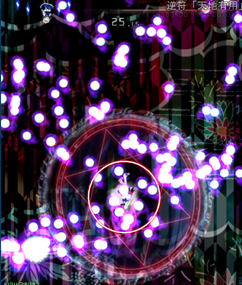
\includegraphics[scale=0.8]{danmaku.png}
\end{wrapfigure}
Our heroine, once again, is on her way to defeat the evil mastermind threating 
our beloved land of fantasy. 


Before reaching her final target, however, our heroine is blocked by one of
the minions of the great evil. Having no interest in dealing with these
valueless targets, our heroine decides to use her time manipulation super power
to stop the time, and quickly move to the other side of the 
rectangular battlefield.

Unfortunately, the evil minion has already released a large amount of circular 
bullets. Even though the heroine can stop the time, she will still die if she 
touches any of the bullets.

Starting from the upper boundary of the battlefield, our heroine wants to
know whether she can safely move to the lower boundary of the battlefield
without touching any of the bullets released by the evil minion.

\InputFile

The first line of input contains two numbers $H, W (1 \le H, W \le 10^6)$,
denoting the height and width of the rectangular battlefield.

The second line of input contains one integer $N (0 \le N \le 2000)$, which
is the number of circular bullets on the battlefield.

The following $N$ lines each contain three numbers $x_i, y_i, r_i$, which are 
the $x$ coordinate, $y$ coordinate, and the radius of the $i$th bullet
($0 \le x_i \le W, 0 \le y_i \le H, 0 < r_i \le 10^6$).

The lower-left corner has coordinate $(0, 0)$ and the upper-right corner
has coordinate $(W, H)$.

The heroine can start from any point on the upper boundary, and can end up on 
any  point on the lower boundary.
It is guaranteed no bullet will touch upper and lower boundaries.
It is also guaranteed bullets will never be tangent with each other or any of
the boundaries.
You can assume our heorine is so small compared to the bullets, and can be
treated as a point.

\OutputFile

A single line either be ``YES YES YES'' if she can safely move to the other side
of the battlefield, or ``NO NO NO'' otherwise.

\Examples

\begin{example}
\exmp{
6.0 4.0
1
2.0 3.0 1.5
}{%
YES YES YES
}%
\exmp{
10.0 6.0
3
2.0 4.0 3.0
3.0 4.0 3.0
4.0 4.0 3.0
}{%
NO NO NO
}%
\end{example}
\end{problem}
